\documentclass[border=12pt]{standalone}
\usepackage[utf8]{inputenc}
\usepackage[T1]{fontenc}
\usepackage{lmodern}
\usepackage{tikz}
\usetikzlibrary{positioning,shapes.geometric,arrows.meta,fit,backgrounds}

\definecolor{mxNavy}{HTML}{12405E}
\definecolor{mxBlue}{HTML}{2A85BE}
\definecolor{mxTask}{HTML}{EEF7FC}
\definecolor{mxLaneA}{HTML}{F7FAFC}
\definecolor{mxLaneB}{HTML}{F2F8FC}
\definecolor{mxLaneC}{HTML}{F8F9FB}

\tikzset{
  startev/.style={circle, draw=green!55!black, fill=green!12, thick, minimum size=6.5mm, inner sep=0pt},
  endev/.style={circle, draw=red!65!black, fill=red!12, ultra thick, minimum size=6.5mm, inner sep=0pt},
  timerev/.style={circle, draw=orange!75!black, fill=orange!10, thick, minimum size=6.5mm, inner sep=1pt, font=\tiny\bfseries},
  task/.style={rectangle, draw=mxBlue, fill=mxTask, thick, rounded corners=3pt, text width=2.7cm, minimum height=1.1cm, align=center, font=\scriptsize\sffamily},
  gtw/.style={diamond, draw=orange!75!black, fill=yellow!15, thick, aspect=1.25, minimum size=7mm, inner sep=1pt, font=\tiny\sffamily\bfseries},
  datastore/.style={cylinder, shape border rotate=90, draw=mxNavy, fill=white, thick, minimum height=0.85cm, minimum width=1.4cm, align=center, font=\tiny\sffamily},
  flow/.style={-{Stealth[length=2.2mm]}, thick, color=mxNavy},
  msg/.style={-{Stealth[length=2.2mm]}, thick, dashed, color=mxBlue},
  lbl/.style={font=\tiny\sffamily\bfseries, text=mxNavy, fill=white, inner sep=1pt}
}

\begin{document}
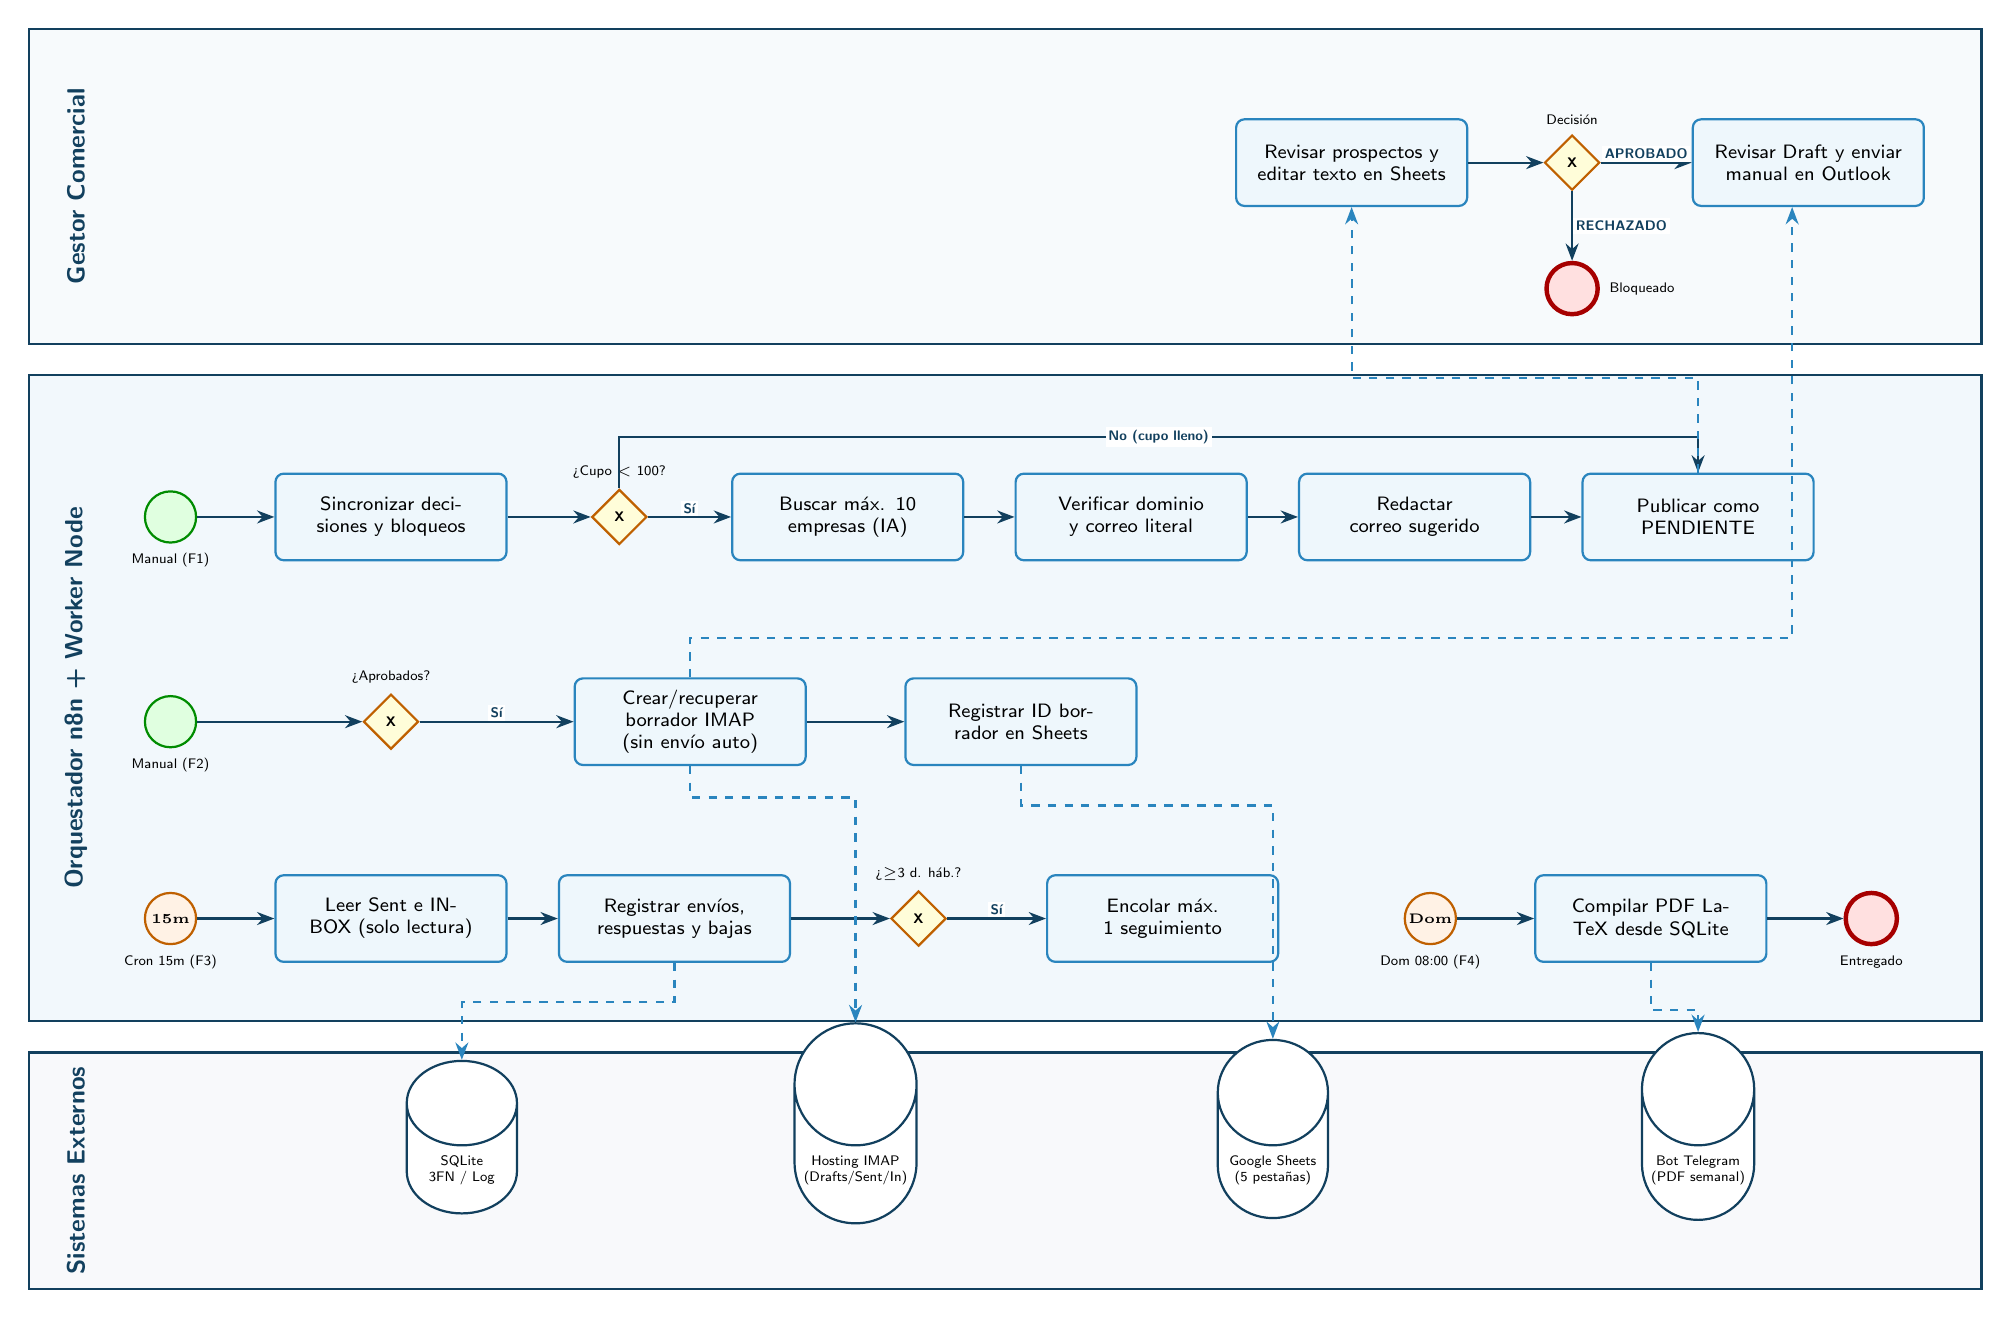
\begin{tikzpicture}

% --- CARRILES FIJOS POR COORDENADAS ---
% Lane 1 (Humano): y = 11.2 .. 15.2
% Lane 2 (n8n + Worker): y = 2.6 .. 10.8
% Lane 3 (Externos): y = -0.6 .. 2.2
\begin{scope}[on background layer]
  \draw[draw=mxNavy, fill=mxLaneA, thick] (-1.0, 11.2) rectangle (23.8, 15.2);
  \node[font=\small\bfseries\sffamily, text=mxNavy, rotate=90] at (-0.4, 13.2) {Gestor Comercial};
  \draw[draw=mxNavy, fill=mxLaneB, thick] (-1.0, 2.6) rectangle (23.8, 10.8);
  \node[font=\small\bfseries\sffamily, text=mxNavy, rotate=90] at (-0.4, 6.7) {Orquestador n8n + Worker Node};
  \draw[draw=mxNavy, fill=mxLaneC, thick] (-1.0, -0.8) rectangle (23.8, 2.2);
  \node[font=\small\bfseries\sffamily, text=mxNavy, rotate=90] at (-0.4, 0.7) {Sistemas Externos};
\end{scope}

% --- CARRIL 1: HUMANO (y = 13.4) ---
\node[task] (humrev) at (15.8, 13.5) {Revisar prospectos y editar texto en Sheets};
\node[gtw, label={[font=\tiny\sffamily]above:Decisión}] (gdec) at (18.6, 13.5) {X};
\node[task] (humsend) at (21.6, 13.5) {Revisar Draft y enviar manual en Outlook};
\node[endev, label={[font=\tiny\sffamily]right:Bloqueado}] (endblk) at (18.6, 11.9) {};

% --- CARRIL 2 - FILA SUPERIOR: FLUJO 1 PROSPECCION (y = 9.0) ---
\node[startev, label={[font=\tiny\sffamily]below:Manual (F1)}] (s1) at (0.8, 9.0) {};
\node[task] (rev1) at (3.6, 9.0) {Sincronizar decisiones y bloqueos};
\node[gtw, label={[font=\tiny\sffamily]above:¿Cupo $<$ 100?}] (gcupo) at (6.5, 9.0) {X};
\node[task] (disc) at (9.4, 9.0) {Buscar máx. 10 empresas (IA)};
\node[task] (verif) at (13.0, 9.0) {Verificar dominio y correo literal};
\node[task] (comp) at (16.6, 9.0) {Redactar correo sugerido};
\node[task] (pub1) at (20.2, 9.0) {Publicar como PENDIENTE};

% --- CARRIL 2 - FILA MEDIA: FLUJO 2 BORRADORES (y = 6.4) ---
\node[startev, label={[font=\tiny\sffamily]below:Manual (F2)}] (s2) at (0.8, 6.4) {};
\node[gtw, label={[font=\tiny\sffamily]above:¿Aprobados?}] (gapr) at (3.6, 6.4) {X};
\node[task] (draft) at (7.4, 6.4) {Crear/recuperar borrador IMAP (sin envío auto)};
\node[task] (pub2) at (11.6, 6.4) {Registrar ID borrador en Sheets};

% --- CARRIL 2 - FILA INFERIOR: FLUJO 3 SEGUIMIENTO + FLUJO 4 REPORTE (y = 3.9) ---
\node[timerev, label={[font=\tiny\sffamily]below:Cron 15m (F3)}] (s3) at (0.8, 3.9) {15m};
\node[task] (imap) at (3.6, 3.9) {Leer Sent e INBOX (solo lectura)};
\node[task] (rec) at (7.2, 3.9) {Registrar envíos, respuestas y bajas};
\node[gtw, label={[font=\tiny\sffamily]above:¿$\ge$3 d. háb.?}] (gseg) at (10.3, 3.9) {X};
\node[task] (qseg) at (13.4, 3.9) {Encolar máx. 1 seguimiento};

\node[timerev, label={[font=\tiny\sffamily]below:Dom 08:00 (F4)}] (s4) at (16.8, 3.9) {Dom};
\node[task] (rep) at (19.6, 3.9) {Compilar PDF LaTeX desde SQLite};
\node[endev, label={[font=\tiny\sffamily]below:Entregado}] (end4) at (22.4, 3.9) {};

% --- CARRIL 3: SISTEMAS EXTERNOS (y = 0.7) ---
\node[datastore] (ds_sql) at (4.5, 0.7) {SQLite\\3FN / Log};
\node[datastore] (ds_im) at (9.5, 0.7) {Hosting IMAP\\(Drafts/Sent/In)};
\node[datastore] (ds_sh) at (14.8, 0.7) {Google Sheets\\(5 pestañas)};
\node[datastore] (ds_tg) at (20.2, 0.7) {Bot Telegram\\(PDF semanal)};

% --- FLECHAS FLUJO 1 ---
\draw[flow] (s1) -- (rev1);
\draw[flow] (rev1) -- (gcupo);
\draw[flow] (gcupo) -- node[lbl, above]{Sí} (disc);
\draw[flow] (disc) -- (verif);
\draw[flow] (verif) -- (comp);
\draw[flow] (comp) -- (pub1);
\draw[flow] (gcupo.north) -- ++(0,0.65) -| node[lbl, pos=0.25]{No (cupo lleno)} (pub1.north);

% --- FLECHAS HUMANO ---
\draw[msg] (pub1.north) -- ++(0,1.2) -| (humrev.south);
\draw[flow] (humrev) -- (gdec);
\draw[flow] (gdec) -- node[lbl, above]{APROBADO} (humsend);
\draw[flow] (gdec) -- node[lbl, right]{RECHAZADO} (endblk);

% --- FLECHAS FLUJO 2 ---
\draw[flow] (s2) -- (gapr);
\draw[flow] (gapr) -- node[lbl, above]{Sí} (draft);
\draw[flow] (draft) -- (pub2);
\draw[msg] (draft.north) -- ++(0,0.5) -| (humsend.250);

% --- FLECHAS FLUJO 3 Y 4 ---
\draw[flow] (s3) -- (imap);
\draw[flow] (imap) -- (rec);
\draw[flow] (rec) -- (gseg);
\draw[flow] (gseg) -- node[lbl, above]{Sí} (qseg);
\draw[flow] (s4) -- (rep);
\draw[flow] (rep) -- (end4);

% --- FLECHAS A EXTERNOS ---
\draw[msg] (rec.south) -- ++(0,-0.5) -| (ds_sql.north);
\draw[msg] (draft.south) -- ++(0,-0.4) -| (ds_im.north);
\draw[msg] (pub2.south) -- ++(0,-0.5) -| (ds_sh.north);
\draw[msg] (rep.south) -- ++(0,-0.6) -| (ds_tg.north);

\end{tikzpicture}
\end{document}
